\documentclass[]{article}
\usepackage[margin={1in}]{geometry}
\usepackage[english]{babel}
\usepackage{datetime}
\usepackage{amsmath}
\usepackage{listings}
\usepackage{verbatim}
\usepackage{fancyhdr}
\usepackage[obeyspaces]{url}
\usepackage{graphicx}
\usepackage{tikz}
\usetikzlibrary{automata, positioning, arrows}
\graphicspath{ {.} }
\newcommand{\class}{TC2006. Programming Languages}
\newcommand{\hwname}{Project 01}
\pagestyle{fancy}
\fancyhf{}
\lhead{\class \\ \hwname}
\rhead{Andrés Alam Sánchez Torres (A00824854) \\ \today}
\lstset{breaklines=true} 

\begin{document}
    \setlength{\headheight}{23.10004pt}
    \addtolength{\topmargin}{-11.10004pt}    

    \noindent
    This document describes the DFA and grammar used to generate the lexical and syntactical analyzer. 
    
    \section{DFA}
    THE DFA recognizes the following lexical elements:

    \begin{itemize}
        \item[] \textbf{INTEGER.} At least one digit followed by zero or more digits. \textbf{Recognized by $q_{101}$}
        \item[] \textbf{REGISTER.} The symbol \# followed by any one letter. \textbf{Recognized by $q_{102}$}
        \item[] \textbf{RESERVED WORD.} One possible reserved word (to be validated in the implementation that is in MOV, ADD, SUB, MUL or DIV) \textbf{Recognized by $q_{103}$}
        \item[] \textbf{EOF.} End of file, specified by the character ';'. \textbf{Recognized by $q_{104}$}
    \end{itemize}
    
    \noindent
    And uses the following definitions:
    \begin{itemize}
        \item[] \textbf{LETTER.} Any \textbf{uppercase} letter.
        \item[] \textbf{DIGIT.} Any digit between 0-9.
        \item[] \textbf{BLANK.} Any whitespace character.
    \end{itemize}

    \begin{center}
        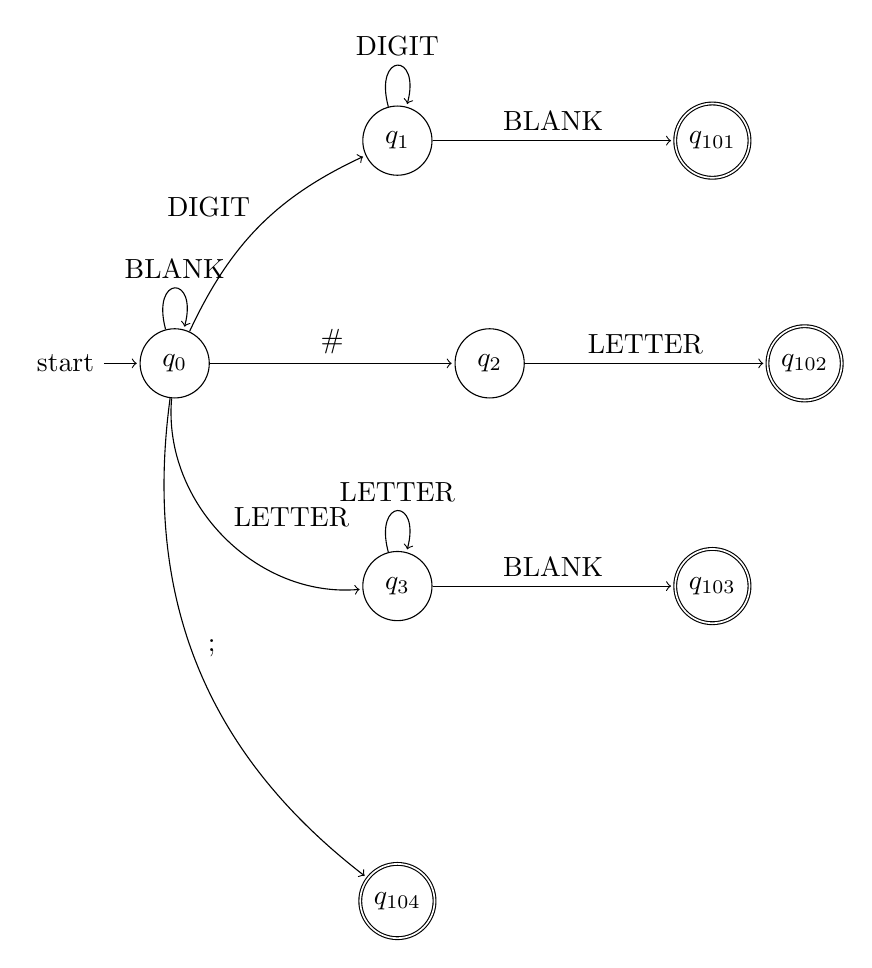
\begin{tikzpicture}[shorten >=1pt,node distance=4cm,on grid,auto] 
            \node[state, initial] (q_0) {$q_0$};
            \node[state] (q_1) [above right=of q_0] {$q_1$}; 
            \node[state] (q_2) [right=of q_0] {$q_2$}; 
            \node[state] (q_3) [below right=of q_0] {$q_3$}; 
            \node[state, accepting] (q_101) [right=of q_1] {$q_{101}$}; 
            \node[state, accepting] (q_102) [right=of q_2] {$q_{102}$}; 
            \node[state, accepting] (q_103) [right=of q_3] {$q_{103}$}; 
            \node[state, accepting] (q_104) [below =of q_3] {$q_{104}$}; 
                \path[->] 
                (q_0) edge [loop above] node {BLANK} (q_0)
                    edge [bend left=20] node {DIGIT} (q_1)
                    edge  node {\#} (q_2)
                    edge [bend right=50] node {LETTER} (q_3)
                    edge [bend right=30] node {;} (q_104)
                (q_1) edge [loop above] node {DIGIT} (q_1)
                    edge node {BLANK} (q_101)
                (q_2) edge node {LETTER} (q_102)
                (q_3) edge [loop above] node {LETTER} (q_3)
                    edge  node  {BLANK} (q_103);
        \end{tikzpicture}
    \end{center}

    \section{Grammar}

    Using the terminals definitions: \\

    \begin{itemize}
        \item[] \verb\REGISTER\ Stands for any register validated by the DFA
        \item[] \verb\INTEGER\ Stands for any integer validated by the DFA
        \item[] \verb\MOV\ The reserved word for movement
        \item[] \verb\OPERATOR\ Any reserved word for operators (ADD, SUB, MUL, DIV) 
    \end{itemize}
    
    
    
    

    \noindent
    The following grammar was designed to match the syntactical rules of the language.\\

    \noindent
    \textit{Notes}:\\
    \textit{O} is short for Operation, \textit{A} short for Assignment. \\

    \begin{gather*}
        S \rightarrow O\ |\ A\ |\ ; \\
        O \rightarrow \mathtt{OPERATOR}\ \mathtt{REGISTER}\ \mathtt{REGISTER} \\
        A \rightarrow \mathtt{MOV}\ A'\ \mathtt{REGISTER} \\
        A' \rightarrow \mathtt{REGISTER}\ |\ \mathtt{INTEGER}\\
    \end{gather*}

  
\end{document}